\documentclass[10pt,aspectratio=169]{beamer}

% --- Theme ---
\usetheme{metropolis}
\metroset{progressbar=none, numbering=fraction, block=fill}
% \usetheme{Boadilla}

% --- Packages ---
\usepackage[utf8]{inputenc}
\usepackage{graphicx}
\usepackage{booktabs}
\usepackage{tikz}
\usetikzlibrary{shapes.geometric, arrows.meta, positioning, calc, fit, backgrounds}
\usepackage{xcolor}
\usepackage{amsmath}
\usepackage{amssymb}
\usepackage{bookmark}
\usepackage{tcolorbox}

% --- Image search paths ---
\graphicspath{
  {../notebooks/images/}
  {../notebooks/images/2025-01-15/}
}

% --- Colors (Tableau-ish, matching deck1) ---
\definecolor{good}{RGB}{44,160,44}
\definecolor{bad}{RGB}{214,39,40}
\definecolor{warn}{RGB}{255,140,0}
\definecolor{accent}{RGB}{31,119,180}

% --- Title metadata ---
\title{Theme Detection - updates II}
\date{May 2026}

\begin{document}

% =====================================================================
\begin{frame}[shrink=5]
  \titlepage
  \vspace{-1.0cm}
  \centering\footnotesize
  Last time: what is a \emph{topic}.\\
  Today: from topics to \emph{themes} --- a working definition, the lifecycle, and how to track them through time.
\end{frame}


% =====================================================================
% A working definition + Vistra
% =====================================================================
\begin{frame}[t]{What is a theme? A working definition (1/5)}
  \footnotesize

  \begin{tcolorbox}[colback=accent!8, colframe=accent, boxrule=0.4pt,
                    left=4pt, right=4pt, top=3pt, bottom=3pt]
    \textbf{Theme} \;=\; \textbf{transient}, \textbf{cross-sectoral} \textbf{exposure}
    created by a shared narrative, structural shift, or value-chain relationship.
  \end{tcolorbox}

  \vspace{0.15cm}
  \begin{columns}[T,onlytextwidth]
    \column{0.32\textwidth}
      \begin{block}{Transient}
        \footnotesize
        Sectors are stable for decades; themes have a \emph{lifecycle} ---
        they emerge, decay, and mutate.
      \end{block}

    \column{0.32\textwidth}
      \begin{block}{Cross-sectoral}
        \footnotesize
        Themes \emph{cut across} sector boundaries, connecting firms
        conventional tools never group together.
      \end{block}

    \column{0.32\textwidth}
      \begin{block}{Exposure}
        \footnotesize
        What matters is the cash-flow link, not vocabulary: a firm that
        \emph{mentions} AI without earning AI revenue is marketing,
        not a thematic investment.
      \end{block}
  \end{columns}

  \vspace{0.30cm}
  \textbf{The Vistra case (2024).}\;
  A US power utility's stock more than tripled --- without an AI pivot.
  Hyperscalers needed electricity; Vistra owned the assets.
  The standard map had a \emph{category} (utility); the market had a \emph{narrative}.\\[0.05cm]
  \(\Rightarrow\) \emph{Markets do not care what a company primarily sells; they care
  about what its future cash flows are exposed to.}

\end{frame}


% =====================================================================
% Lifecycle
% =====================================================================
\begin{frame}[t]{Theme lifecycle: clean energy 2018--2024 (2/5)}
  \footnotesize

  \begin{center}
  \resizebox{0.98\textwidth}{!}{%
  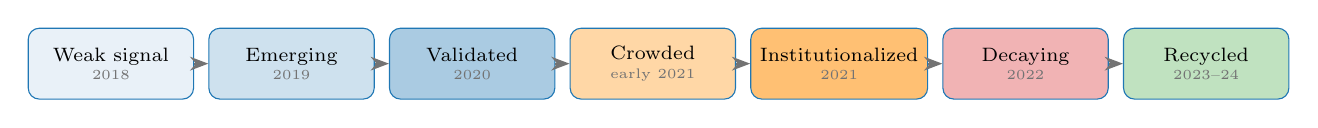
\begin{tikzpicture}[
      node distance=0.05cm,
      stage/.style={rectangle, rounded corners, draw=accent, line width=0.4pt,
                    minimum width=2.1cm, minimum height=0.9cm,
                    font=\scriptsize, align=center},
      arr/.style={-Stealth, thick, draw=black!55}
    ]
    \node[stage, fill=accent!10]  (a) {Weak signal\\[-0.05cm]\textcolor{black!55}{\tiny 2018}};
    \node[stage, fill=accent!22, right=0.18cm of a]  (b) {Emerging\\[-0.05cm]\textcolor{black!55}{\tiny 2019}};
    \node[stage, fill=accent!38, right=0.18cm of b]  (c) {Validated\\[-0.05cm]\textcolor{black!55}{\tiny 2020}};
    \node[stage, fill=warn!35,    right=0.18cm of c]  (d) {Crowded\\[-0.05cm]\textcolor{black!55}{\tiny early 2021}};
    \node[stage, fill=warn!55,    right=0.18cm of d]  (e) {Institutionalized\\[-0.05cm]\textcolor{black!55}{\tiny 2021}};
    \node[stage, fill=bad!35,     right=0.18cm of e]  (f) {Decaying\\[-0.05cm]\textcolor{black!55}{\tiny 2022}};
    \node[stage, fill=good!30,    right=0.18cm of f]  (g) {Recycled\\[-0.05cm]\textcolor{black!55}{\tiny 2023--24}};
    \draw[arr] (a) -- (b);
    \draw[arr] (b) -- (c);
    \draw[arr] (c) -- (d);
    \draw[arr] (d) -- (e);
    \draw[arr] (e) -- (f);
    \draw[arr] (f) -- (g);
  \end{tikzpicture}}
  \end{center}

  \vspace{0.15cm}
  \begin{columns}[T,onlytextwidth]
    \column{0.5\textwidth}
      \begin{block}{Where alpha lives}
        \footnotesize
        Earliest stages --- \textbf{weak signal} and \textbf{emerging} ---
        when a story is detectable but not priced.
        By the time a thematic ETF reaches the market, the founding
        observation has often \emph{already been priced}.
      \end{block}

    \column{0.5\textwidth}
      \begin{block}{What changes per stage}
        \footnotesize
        Granularity, breadth of coverage, and the \emph{type of signal}
        that moves the price:
        research \(\rightarrow\) flows \(\rightarrow\) index inclusion
        \(\rightarrow\) liquidation.
      \end{block}
  \end{columns}

\end{frame}


% =====================================================================
% Pipeline
% =====================================================================
\begin{frame}[t]{From topic to portfolio: the five transitions (3/5)}
  \footnotesize

  \begin{center}
  \resizebox{0.98\textwidth}{!}{%
  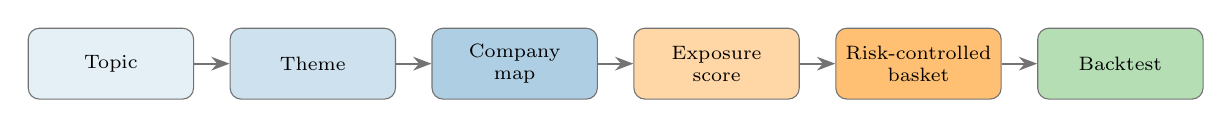
\begin{tikzpicture}[
      box/.style={rectangle, rounded corners, draw=black!55, line width=0.4pt,
                  minimum width=2.1cm, minimum height=0.9cm,
                  font=\scriptsize, align=center},
      arr/.style={-Stealth, thick, draw=black!55}
    ]
    \node[box, fill=accent!12] (t)                           {Topic};
    \node[box, fill=accent!22, right=0.45cm of t] (h)        {Theme};
    \node[box, fill=accent!36, right=0.45cm of h] (m)        {Company\\ map};
    \node[box, fill=warn!35,   right=0.45cm of m] (e)        {Exposure\\ score};
    \node[box, fill=warn!55,   right=0.45cm of e] (b)        {Risk-controlled\\ basket};
    \node[box, fill=good!35,   right=0.45cm of b] (k)        {Backtest};
    \draw[arr] (t) -- (h);
    \draw[arr] (h) -- (m);
    \draw[arr] (m) -- (e);
    \draw[arr] (e) -- (b);
    \draw[arr] (b) -- (k);
  \end{tikzpicture}}
  \end{center}

  \vspace{0.15cm}
  \begin{columns}[T,onlytextwidth]
    \column{0.55\textwidth}
      \textbf{Each arrow is a research bet.}\\[0.05cm]
      \begin{itemize}\setlength\itemsep{0.04cm}
        \item Topic \(\to\) \emph{Theme}: meaning, durability, investability.
        \item Theme \(\to\) \emph{Map}: which firms? value-chain reasoning, not vocabulary match.
        \item Map \(\to\) \emph{Exposure}: graded score, not membership.
        \item Exposure \(\to\) \emph{Basket}: risk targeting, sector neutralisation.
        \item Basket \(\to\) \emph{Backtest}: leakage-free, point-in-time.
      \end{itemize}

    \column{0.43\textwidth}
      \begin{block}{Why the chain matters}
        \footnotesize
        A \textbf{cluster of news is not a portfolio};
        \textbf{a topic is not alpha}.
        Most apparent alpha in naive setups is the model trading on
        documents the live system \emph{could not have seen} at decision time.
      \end{block}
  \end{columns}

\end{frame}


% =====================================================================
% Tracking through time
% =====================================================================
\begin{frame}[t]{Tracking themes over time (4/5)}
  \footnotesize

  \textbf{Static} models find clusters \emph{after the fact}.
  \textbf{Dynamic} models show that topic vocabulary moves.
  An \textbf{online / candidate-theme} system answers the harder question:
  is today's cluster the \emph{continuation} of yesterday's,
  a \emph{split}, a \emph{merger}, or genuinely \emph{new}?

  \vspace{0.20cm}
  \begin{columns}[T,onlytextwidth]
    \column{0.49\textwidth}
      \begin{block}{Identity vs.\ vocabulary drift}
        \footnotesize
        Topic \emph{identity} stays fixed; \emph{vocabulary} moves.
        D-ETM-style models share embedding structure so semantically
        related words drift together --- rather than every rare word
        having to earn its own history.
      \end{block}

      \begin{block}{Online tracking (BERTrend-style)}
        \footnotesize
        Refit/extend the global map only with documents
        \emph{known as of the decision date}.
        Keep an \textbf{outlier buffer} for proto-themes that have not
        yet stabilised into a cluster.
      \end{block}

    \column{0.49\textwidth}
      \begin{block}{Four transitions to detect}
        \footnotesize
        \begin{tabular}{@{}ll@{}}
          \textbf{Continuation} & same theme, drifted vocabulary \\
          \textbf{Split}        & one theme branches into several \\
          \textbf{Merge}        & several threads converge \\
          \textbf{Birth}        & genuinely new candidate theme \\
        \end{tabular}
      \end{block}

      \begin{block}{False positives to guard against}
        \footnotesize
        Duplicate documents, a new source added to the corpus,
        ticker / OCR errors, seasonal language,
        coordinated manipulation, model retraining itself.
      \end{block}
  \end{columns}

\end{frame}


% =====================================================================
% Embedding upgrades for the sector-aware BERTopic pipeline
% =====================================================================
\begin{frame}[t]{Better embeddings for the sector-aware pipeline (5/5)}
  \footnotesize

  \textbf{Today (\texttt{0.3-themes.ipynb}).}\;
  FinLang embeds news headlines and 173 ICB subsector definitions
  $\rightarrow$ averaged into \textbf{45 sector centroids}
  $\rightarrow$ BERTopic on headline embeddings
  $\rightarrow$ cosine vs centroids
  $\rightarrow$ \emph{aligned} ($\max\!\cos \!\ge\! \tau_{\text{cov}}\!=\!0.30$) / \emph{novel}.\;
  Last run: 22 aligned, 18 novel.\;
  \emph{Encoder choice is the single biggest lever ---
  a domain-tuned swap typically beats any pooling or preprocessing tweak.}

  \vspace{0.10cm}
  \begin{columns}[T,onlytextwidth]
    \column{0.49\textwidth}
      \begin{block}{Encoder candidates (biggest lever)}
        \footnotesize
        \begin{itemize}\setlength\itemsep{0.04cm}
          \item \textbf{FinLang} --- current baseline (finance-tuned).
          \item \textbf{FinBERT-MPNet} --- head-to-head with FinLang on the same 45-sector cosine task.
          \item \textbf{LoRA on \texttt{bge-large}} --- strong general encoder lightly adapted to financial text; cheaper to maintain than full domain pretraining.
        \end{itemize}
      \end{block}

    \column{0.49\textwidth}
      \begin{block}{Pooling \& preprocessing}
        \footnotesize
        \begin{itemize}\setlength\itemsep{0.04cm}
          \item \textbf{Sum-pool / concat last 4 hidden layers} of the SBERT encoder, instead of default last-layer mean pooling --- cited \emph{$+10$--$20\%$ relative} on topic diversity \& coherence on news corpora.
          \item \textbf{Stop-word removal at embedding time}, not only at the c-TF-IDF stage --- small alone, compounds with the rest.
        \end{itemize}
      \end{block}
  \end{columns}

  \vspace{0.15cm}
  \textbf{Evaluation on the current pipeline.}\;
  Topic coherence (NPMI, $C_v$) and diversity on BERTopic output;
  sector separation on the 45-centroid axis ---
  median \texttt{max\_cos} for \emph{aligned} vs \emph{novel}, and the share of themes crossing $\tau_{\text{cov}}$.

\end{frame}


\end{document}
